% Author: Seongjin Lee
% Hanyang University, Seoul, Korea
% esos.hanyang.ac.kr
% 2016-09-20
% note: some slides are adopted from  \url{www.cs.stevens.edu/~jschauma/631A/}
% https://github.com/resourceful/lecture_sysprog/

\documentclass[newPxFont,sthlmFooter,nooffset]{beamer}
\usepackage{kotex}
%\usetheme{sthlm}
\usepackage{../beamer_template/beamerthemesthlm}
\hypersetup{pdfauthor={Seongjin Lee (insight@gnu.ac.kr)},
            pdfsubject={Lecture Note: System Programming},
            pdfkeywords={Lecture Note, System Programming, class, (under)graduate},
            pdfmoddate={D: \pdfdate},
            pdfcreator={Seongjin Lee}}

%\setbeamertemplate{footline}[text line]{%
%    \parbox{\linewidth}{\vspace*{-8pt} \insertsectionhead  \hfill\insertshortauthor\hfill\insertpagenumber}}
%\setbeamertemplate{navigation symbols}{}




\title{System Programming}
\subtitle{Topic 11: Sockets}
\author[SJL]{Seongjin Lee}
\institute{\href{mailto:insight@gnu.ac.kr}{insight@gnu.ac.kr}\\\url{http://open.gnu.ac.kr}\\Systems Research Lab.\\Gyeongsang National University}
\date{\today}

\begin{document}



\frame[plain]{\titlepage}

\frame[t]{\frametitle{Table of contents}\tableofcontents}


%---------------------------------------------------------

\section{Sockets}

\begin{frame}[t, fragile]
  \frametitle{Sockets}
Socket netwok IPC interface that allow to communicate with other process
\begin{itemize}
\item either on the same machine or
\item on different machine over a network
\end{itemize}
\end{frame}


\begin{frame}[t, fragile]
  \frametitle{Client-Server Setup}
Sockets are used as follows:
\begin{itemize}
\item Applications create a socket
\item Server bind its sockets to well-known addresss
\item locate server sockets via its well-known address and communicate with the server
\end{itemize}


\end{frame}


\begin{frame}[t, fragile]
  \frametitle{Socket syscall}
Sockets are created using the socket syscall which returns a file descriptor to be used for further operations on the underlying socket:

\begin{codedef}
#include <sys/socket.h>
fd = socket(domain, type, protocol)
// Returns: file descriptor on success, -1 on error
\end{codedef}


\begin{itemize}
\item Domain: \texttt{AF\_UNIX}, \texttt{AF\_INET}, \texttt{AF\_INET6}
\item Each communication domain determines
  \begin{itemize}
  \item how to identify a socket, that is the syntax and semantics of socket well-known addresses
  \item the communication range, e.g. single or multiple hosts
  \end{itemize}
\end{itemize}

\end{frame}


\begin{frame}[t, fragile]
  \frametitle{Communication Domains}
  \begin{table}
    \centering
    \begin{tabular}{m{1.5cm} | m{2cm} | m{2cm} | m{2cm} | m{2cm}}
      domain & range & transport & address format & address C struct \\ \hline
      \texttt{AF\_UNIX} & same host & kernel & pathname & \texttt{sockaddr\_un} \\ \hline
      \texttt{AF\_INET} & any host w/ IPv4 connectivity & IPv4 stack & 32-bit IPv4 address + 16bit port number & \texttt{sockaddr\_in} \\ \hline
      \texttt{AF\_INET6} & any host w/ IPv6 connectivity & IPv6 stack & 128-bit IPv6 address + 16bit port number  & \texttt{sockaddr\_in6} \\
    \end{tabular}
  \end{table}

\end{frame}


\begin{frame}[t, fragile]
  \frametitle{Socket Types}
Socket types offer different IPC features

\begin{table}
  \centering
  \begin{tabular}{c | c | c}
    Feature & \texttt{SOCK\_STREAM} & \texttt{SOCK\_DGRAM} \\ \hline
    realiable delivery & yes & no \\ \hline
    fixed length & no & yes \\ \hline
    connection-oriented & yes & no \\
  \end{tabular}
\end{table}
\end{frame}


\begin{frame}[t, fragile]
  \frametitle{Stream Sockets : \texttt{SOCK\_STREAM}}
Stream sockets provide communication channels which are:
\begin{itemize}
\item byte-stream: communication happens as a continuous stream of bytes
\item reliable: either data transmitted arrive at destination, or the sender gets an error
\item bidirectional: between two sockets, data can be transmitted in either direction
\item connection-oriented: sockets operate in connected pairs, each connected pair of sockets denotes a communication context, isolated from other pairs
\end{itemize}

\end{frame}


\begin{frame}[t, fragile]
  \frametitle{Datagram Sockets : \texttt{SOCK\_DGRAM}}
Datagram sockets provide communication channels which are:
\begin{itemize}
\item message-oriented: data is exchanged at the granularity of messages that peers send to one another; Message length is fixed
\item non-reliable: messages can get lost. Also:
  \begin{itemize}
  \item messages can arrive out of order
  \item messages can be duplicated and arrive multiple times
  \end{itemize}
  It is up to applications to detect these scenarios and react
  (e.g. by re-sending messages after a timeout, adding sequence
  numbers, etc.).
\item connection-less: sockets do not need to be connected in pairs to be used; you can send a message to, or receive a message from, a socket without connecting to it beforehand
\end{itemize}

\end{frame}


\begin{frame}[t, fragile]
  \frametitle{Binding sockets to a well-known address}
To allow connections from others, we need to bind sockets to well-known addresses using bind:
\begin{codedef}
#include <sys/socket.h>
int bind(int sockfd, const struct sockaddr *addr, socklen_t addrlen);
// Returns: 0 on success, -1 on error
\end{codedef}
\begin{itemize}
\item \texttt{sockfd} references the socket we want to bind
\item \texttt{sockaddr} \texttt{addr} and \texttt{addrlen} depends on the socket domain
\end{itemize}
\end{frame}


\begin{frame}[t, fragile]
  \frametitle{Generic Socket Address Structure}
An address identifies a socket endpoint in a particular communication domain. The address format is specific to the particular domain.

\begin{codedefnb}
 struct sockaddr {
     sa_family_t  sa_family;    /* address family */
     char         sa_data[14];  /* socket address (size varies with the socke domain) */
};
\end{codedefnb}
\begin{itemize}
\item Each socket domain has its own variant of \texttt{sockaddr}
\item user has to fill the domain-specific struct and cast it to \texttt{struct sockaddr} before passing it to bind
\end{itemize}
\end{frame}


\begin{frame}[t, fragile]
  \frametitle{Stream socket syscalls - overview}
\begin{columns}
\begin{column}{0.5\textwidth}
  \begin{figure}[h]
    \centering
    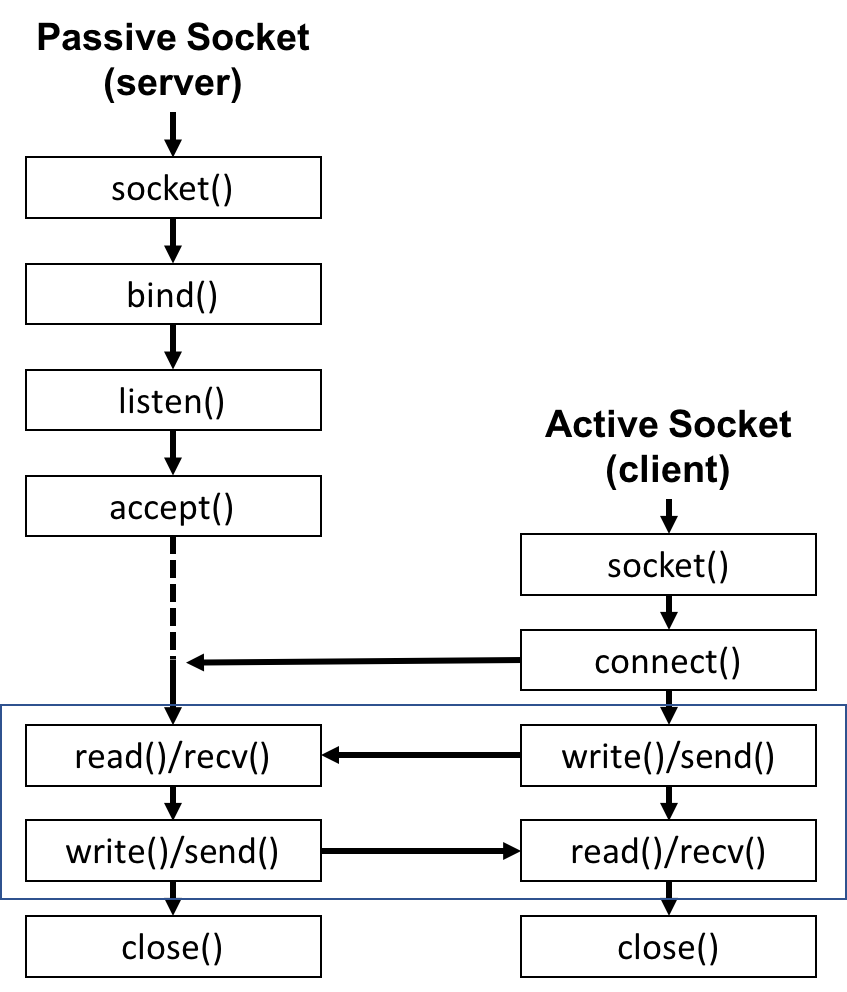
\includegraphics[width=\linewidth]{figures/fig_socket_syscall.png}
  \end{figure}
\end{column}
\begin{column}{0.5\textwidth}
 ``Server'' and ``Client'' are ambiguous terms

Passive and Active sockets are more precise
\begin{itemize}
\item sockets are created active : \texttt{listen()} makes them passive
\item \texttt{connect()} performs an active open
\item \texttt{accept()} performs a passive open
\end{itemize}
\end{column}
\end{columns}


\end{frame}


\begin{frame}[t, fragile]
  \frametitle{Active to passive sockets}
\texttt{listen()} turns an active socket into a passive one, allowing it to accept incoming connections

\begin{codedef}
#include <sys/socket.h>
int listen(int sockfd, int backlog);
// Returns: 0 on success, -1 on error
\end{codedef}

\texttt{backlog} specifies the maximum number of pending connections that the passive socket will keep
\begin{itemize}
\item active opens may be performed before the matching passive ones
\item not yet accepted connections are called pending
\item \texttt{pending < backlog} connect succeeds immediately
\item \texttt{pending >= backlog} connect blocks waiting for an accept
\end{itemize}

\end{frame}


\begin{frame}[t, fragile]
  \frametitle{Accepting Connections}
You can accept connections (i.e. perform a passive open) with:
\begin{codedef}
#include <sys/socket.h>
int accept(int sockfd, struct sockaddr *addr, socklen_t *addrlen);
// Returns: file descriptor on success, -1 on error
\end{codedef}
\begin{itemize}
\item If the corresponding active open hasn’t been performed yet, accept blocks waiting for it.
\item When the active open happens---or if it has already happened---accept returns a new socket connected to the peer socket.
\item The original socket remains available and can be used to accept other connections.
\end{itemize}
\end{frame}


\begin{frame}[t, fragile]
  \frametitle{Connecting the socket}
you connect (i.e. perform an active open) with:

\begin{codedef}
#include <sys/socket.h>
int connect(int sockfd, struct sockaddr *addr, socklen_t addrlen);
// Returns: 0 on success, -1 on error
\end{codedef}
\begin{itemize}
\item \texttt{sockfd} is your own socket, to be used as your endpoint of the connection
\item \texttt{addr/addrlen} specify the well-known address of the peer you want to connect to, and are given in the same format of bind parameters
\end{itemize}
\end{frame}


\begin{frame}[t, fragile]
  \frametitle{Creating Sockets}

\begin{codedefnb}
int listenfd;   /* Socket to listen on */
int optval = 1; /* Used by setsockopt() below */
if ((listenfd = socket(AF_INET, SOCK_STREAM, 0)) < 0) {
     perror("Cannot create socket");
     exit(1);
}

/* Allow this socket to reuse a port number */
if (setsockopt(listenfd, SOL_SOCKET, SO_REUSEADDR,
           (const void*)&optval, sizeof(int)) < 0) {
     perror("Cannot set SO_REUSEADDR socket option");
     exit(1);
}
\end{codedefnb}
\begin{itemize}
\item create a socket: \texttt{socket()} system call
\item use \texttt{setsockopt()} to permit socket to reuse the server port number
\end{itemize}
\end{frame}


\begin{frame}[t, fragile]
  \frametitle{Binding Listening}
\begin{codedefnb}
struct sockaddr_in server_addr;
bzero(&server_addr, sizeof(server_addr)); /* Zero out the server address */
server_addr.sin_family = AF_INET;
/* Listen for connections from any client on the Internet. */
server_addr.sin_addr.s_addr = htonl(INADDR_ANY);
server_addr.sin_port = htons(80); /* Listen for connections on port 80 */
/* Bind socket to address */
if (bind(listenfd, (struct sockaddr *)&server_addr,
                          sizeof(server_addr)) < 0) {
     perror("Cannot bind socket");
     exit(1);
}
/* Listen for incoming connections. Use listen queue length of 10. */
if (listen(listenfd, 10) < 0) {
     perror("Cannot listen");
     exit(1);
}
\end{codedefnb}
\begin{itemize}
\item \texttt{bind()} the socket to the port you want to listen on
  \begin{itemize}
  \item  \texttt{INADDR\_ANY} to accept connections from any IP address
  \end{itemize}
\item \texttt{listen()} for incoming connections
\end{itemize}
\end{frame}


\begin{frame}[t, fragile]
  \frametitle{Accept Connection}
\begin{codedefnb}
int clifd;
struct sockaddr_in client_addr;
int client_addr_len = sizeof(client_addr);
while (1) {
     clifd = accept(listenfd,
     (struct sockaddr *)&client_addr,
                   (socklen_t*)&client_addr_len);
     /* Process connection here */
     do_something(clifd);
     close(clifd);
}
\end{codedefnb}
\begin{itemize}
\item The server spins in a loop doing the following:
  \begin{itemize}
  \item Call accept() to accept an incoming connection from the
    Internet (blocks until a connection is received)
  \item Process the connection close() the client socket
  \end{itemize}
\item \texttt{accept()} returns a new file descriptor representing the socket for the new connection.
\end{itemize}
\end{frame}


\begin{frame}[t, fragile]
  \frametitle{Process the connection}
\begin{codedefnb}
rio_t rio; /* Use the RIO libraries to do I/O */
    Rio_readinitb(&rio, clifd);
/* Read lines from the client */
while ((n = Rio_readlineb(&rio, buf, BUFSIZE)) != 0) {
      fprintf(stderr, "Read line from client: %s\n", buf);
      if (strcmp(buf, "\r\n") == 0) {
        // Got a blank line, means request is done.
break; }
}
    /* Send the client some HTML */
    sprintf(buf, "<html><body><b>Hello from my awesome web server.</b><p>You are
coming from %s with IP address %s.<br>Have a nice day!</body></html>\n",
     hostname, hostip);
    /* Send data back to client */
Rio_writen(clifd, buf, strlen(buf));
\end{codedefnb}
\end{frame}


\begin{frame}[t, fragile]
  \frametitle{More info on}

\url{http://www.binarytides.com/socket-programming-c-linux-tutorial/}
\end{frame}

%---------------------------------------------------------

\section{Last Words}

\begin{frame}[t]
  \frametitle{Last Words}

\begin{itemize}
\item prepare for the exam
\end{itemize}
\end{frame}


\end{document}
